%%%%%%%%%%%%%%%%%%%%%%%%%%%%%%%%%%%%%%%%%
% Diaz Essay
% LaTeX Template
% Version 2.0 (13/1/19)
%
% This template originates from:
% http://www.LaTeXTemplates.com
%
% Authors:
% Vel (vel@LaTeXTemplates.com)
% Nicolas Diaz (nsdiaz@uc.cl)
%
% License:
% CC BY-NC-SA 3.0 (http://creativecommons.org/licenses/by-nc-sa/3.0/)
%
%%%%%%%%%%%%%%%%%%%%%%%%%%%%%%%%%%%%%%%%%

%----------------------------------------------------------------------------------------
%	PACKAGES AND OTHER DOCUMENT CONFIGURATIONS
%----------------------------------------------------------------------------------------
\documentclass[11pt]{diazessay} % Font size (can be 10pt, 11pt or 12pt)
\usepackage{graphicx}
\usepackage{array}
\usepackage{tabularx}
\usepackage{float}
\usepackage{csquotes}
\usepackage{csquotes}
\usepackage{listings}
\usepackage{xcolor}
\lstset { %
    language=C++,
    backgroundcolor=\color{black!5}, % set backgroundcolor
    basicstyle=\footnotesize,% basic font setting
    breaklines=true,
}
%----------------------------------------------------------------------------------------
%	TITLE SECTION
%----------------------------------------------------------------------------------------

\title{\textbf{Trabajo Práctico} \\ {\Large\itshape Analisis de Circuitos}} % Title and subtitle

\author{\textbf{Cotarelo Rodrigo} \\ \textit{Facultad de Ingeniería, Universidad de Buenos Aires}} % Author and institution

\date{\today} % Date, use \date{} for no date



%----------------------------------------------------------------------------------------

\begin{document}

\vbox{
    \centering
    \maketitle %this typesets the contents of \title, \author and \date
    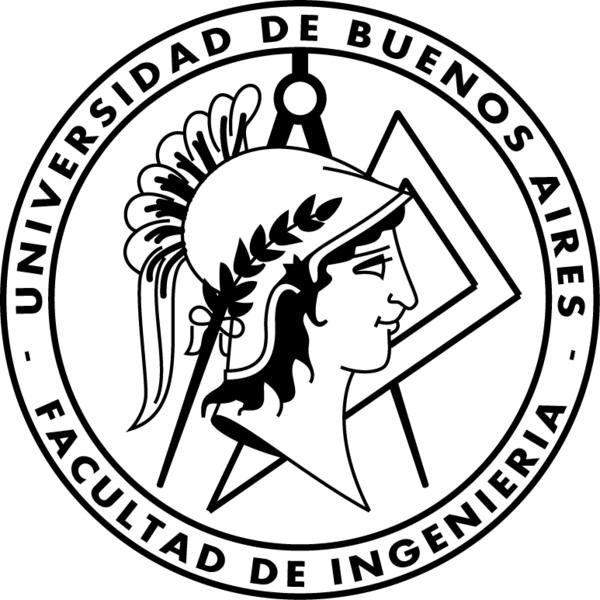
\includegraphics[width=0.5\textwidth]{Figures/fiuba.png}
}


%----------------------------------------------------------------------------------------
%	ESSAY BODY
%----------------------------------------------------------------------------------------
\newpage
\section*{Definit tipo de filtro}

\begin{equation}
H(s) = \frac{6,317*10^8*s^2}{s^4 + 3,554*10^4*s^3 + 1,895*10^9*s^2 + 2,245*10^{13}*s + 3,99*10^{17}} 
\end{equation}

En un primer analisis podemos indentificar que se trata de un filtro pasa-banda ya que tendiendo a infinito o menos infinito podemos 
ver que la transferencia es cero. Ademas como tenemos un cero en cero sabemos que hay una subida de ganancia que luego tiene que ser atenuada y es por esto
que lo podemos diferenciar de un pasa-bajos por ejemplo.\\
\\
Esta compuesto por 4 polos los cuales son dos pares complejos conjugados:
\begin{itemize}
	\item -12002.32+34212.9j\\
	\item -12002.32-34212.9j\\
	\item -5767.68+16439.38j\\
	\item -5767.68-16439.38j
\end{itemize}

Como los polos complejos conjugadores se consideran como un polo real doble y sabiendo como se conforma el diagrama asintotico sabemos que existen
dos caidas en la transferencia (una por cada polo doble) con pendiente -40db y una subida de 40db gracias al cero doble. Esto se corresponde con el
grafico de pasabanda que esperamos obtener.

\newpage
\section*{Simulacion}
\begin{itemize}
\item Diagrama de Bode de modulo y fase
Podemos confirmar lo explicado anteriormente. El gráfico muestra claramente la subida de 40 db por década que después se compensa con el primer polo doble generando una meseta y en el segundo polo doble se produce la caída de -40 db por década.\\
\begin{figure}[h]
	\centering
	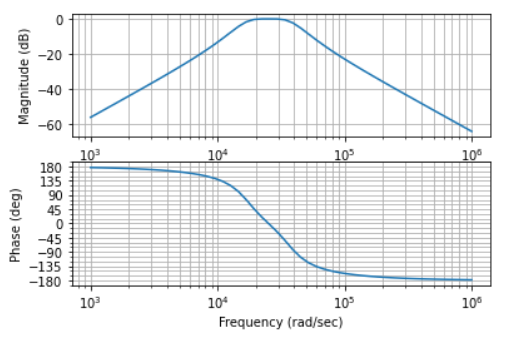
\includegraphics[width=\textwidth]{Bode.png}
\caption{Diagrama de Bode de modulo y fase}
\end{figure}\\
\newpage
\item Respuesta al escalon
\begin{figure}[h]
	\centering
	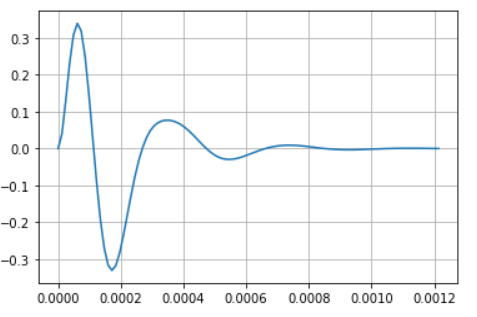
\includegraphics[width=\textwidth]{Respuesta_al_escalon.png}
\caption{Respuesta al escalon.}
\end{figure}
\newpage
\item Respuesta al impulso
\begin{figure}[h]
	\centering
	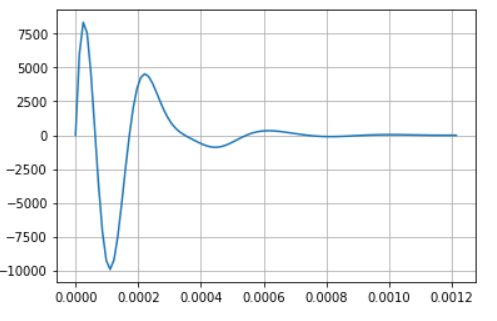
\includegraphics[width=\textwidth]{Respuesta_al_impulso.png}
\caption{Respuesta al impulso.}
\end{figure}

\end{itemize}

%------------------------------------------------

\end{document}
